% Created 2018-03-01 jue 11:05
\documentclass[presentation,aspectratio=1610]{beamer}
\usepackage[utf8]{inputenc}
\usepackage[T1]{fontenc}
\usepackage{fixltx2e}
\usepackage{graphicx}
\usepackage{longtable}
\usepackage{float}
\usepackage{wrapfig}
\usepackage{rotating}
\usepackage[normalem]{ulem}
\usepackage{amsmath}
\usepackage{textcomp}
\usepackage{marvosym}
\usepackage{wasysym}
\usepackage{amssymb}
\usepackage{hyperref}
\tolerance=1000
\usepackage{khpreamble}
\usepackage{algorithm}
\usepackage{hyperref}
\usepackage{framed}
\usepackage[noend]{algpseudocode}
\usepackage{tikz,pgf}
\usetikzlibrary{shapes.geometric}
\newcommand{\sign}{\mathrm{sign}}
\renewcommand{\transp}{^{\mathrm{T}}}
\DeclareMathOperator*{\argmin}{arg\,min}
\DeclareMathOperator*{\argmax}{arg\,max}
\DeclareMathOperator*{\EXP}{E}
\DeclareMathOperator*{\COV}{cov}
\definecolor{uured}{rgb}{0.65, 0., 0.}
\DeclareMathOperator*{\E}{E}
\DeclareMathOperator*{\Var}{Var}
\usetheme{default}
\author{Kjartan Halvorsen}
\date{}
\title{Gazebo and ROS  - part 2}
\hypersetup{
  pdfkeywords={},
  pdfsubject={},
  pdfcreator={Emacs 24.5.1 (Org mode 8.2.10)}}
\begin{document}

\maketitle

\section{Introduction}
\label{sec-1}
\begin{frame}[label=sec-1-1]{Overview}
\begin{enumerate}
\item Position control of the Pioneer2dx robot
\item Adding a depth camera to the robot
\item Using the parameter server
\item Ideas for coming ROS seminars
\end{enumerate}
\end{frame}

\begin{frame}[label=sec-1-2]{Sources}
\begin{itemize}
\item \url{http://gazebosim.org/}
\item \url{http://gazebosim.org/tutorials/?tut=ros_comm}
\item \url{http://docs.ros.org/kinetic/api/gazebo_msgs/html/index-msg.html}
\item \url{http://gazebosim.org/tutorials?tut=ros_depth_camera&cat=connect_ros}
\end{itemize}
\end{frame}


\section{Simulating a robot in Gazebo}
\label{sec-2}

\begin{frame}[fragile,label=sec-2-1]{A simple controller (reusing code)}
 Download the code

\begin{verbatim}
~$ roscd pioneer_gazebo/src
~/catkin_ws/src/pioneer_gazebo/src$ wget \
> http://alfkjartan.github.io/files/robot_controller.cpp

~/catkin_ws/src/pioneer_gazebo/src$ cd ..
~/catkin_ws/src/pioneer_gazebo$ wget \
> http://alfkjartan.github.io/files/CMakeLists.txt
\end{verbatim}
\end{frame}


\begin{frame}[fragile,label=sec-2-2]{A simple controller - usage}
 Build the package etc, then

\begin{verbatim}
~$ rosrun pioneer_gazebo pioneer_controller
\end{verbatim}
\end{frame}

\section{Adding a depth camera}
\label{sec-3}
\begin{frame}[label=sec-3-1]{Adding a depth camera to the pioneer}
\begin{enumerate}
\item Make a new gazebo depth camera that publishes its data to ROS topics (add plugin)
\item Attach the depth camera to the pioneer2dx robot
\end{enumerate}
\end{frame}
\begin{frame}[label=sec-3-2]{Add ROS plugin to depth camera}
\begin{enumerate}
\item In gazebo, insert a depth camera from the model database
\item Quit gazebo
\end{enumerate}
\end{frame}

\begin{frame}[fragile,label=sec-3-3]{Add ROS plugin to depth camera, contd}
 We now have the definition of the depth camera stored locally. Let's make a copy and modify.

\begin{enumerate}
\setcounter{enumi}{2}
\item Create a copy of the depth camera model
\begin{verbatim}
~$ cd ~/.gazebo/models
~$ cp -R depth_camera ros_depth_camera
\end{verbatim}
\item Change the name of the model in the \texttt{model.config} file and the \texttt{model.sdf} file.
\item Add the \texttt{<plugin>} tag in the \texttt{model.sdf} file
\end{enumerate}
\end{frame}

\begin{frame}[fragile,label=sec-3-4]{Add ROS plugin to depth camera, contd}
 \begin{enumerate}
\setcounter{enumi}{6}
\item Add the \texttt{<plugin>} tag in the \texttt{model.sdf} file right before thex closing \texttt{</sensor>} tag
\begin{verbatim}
<plugin name="camera_plugin" filename="libgazebo_ros_openni_kinect.so">
  <baseline>0.2</baseline>
  <alwaysOn>true</alwaysOn>
  <updateRate>0.0</updateRate>
  <cameraName>camera</cameraName>
  <imageTopicName>/camera/depth/image_raw</imageTopicName>
  <cameraInfoTopicName>/camera/depth/camera_info</cameraInfoTopicName>
  <depthImageTopicName>/camera/depth/image_raw</depthImageTopicName>
  <depthImageInfoTopicName>/camera/depth/camera_info</depthImageInfoTopicName>
  <pointCloudTopicName>/camera/depth/points</pointCloudTopicName>
  <frameName>camera_link</frameName>
  ...
  </plugin>
\end{verbatim}
\end{enumerate}
\end{frame}

\begin{frame}[label=sec-3-5]{Adding a depth camera to the pioneer}
\begin{enumerate}
\item Make a new gazebo depth camera that publishes its data to ROS topics (add plugin)
\item \alert{Attach the depth camera to the pioneer2dx robot}
\end{enumerate}
\end{frame}

\begin{frame}[fragile,label=sec-3-6]{Attaching the depth camera}
 Modify the \texttt{pioneer.world} file
\begin{verbatim}
~$ roscd pioneer_gazebo/worlds
~/catkin_ws/src/pioneer_gazebo/worlds$ gedit pioneer.world
\end{verbatim}

Add the depth camera to the definition of the pioneer model. Right before ending \texttt{</model>} tag:
\begin{verbatim}
<include>
  <uri>model://ros_depth_camera</uri>
  <pose>0.2 0 0.2 0 0 0</pose>
</include>
<joint name="depth_camera_joint" type="fixed">
  <child>ros_depth_camera::link</child>
  <parent>chassis</parent>
</joint>
\end{verbatim}
\end{frame}

\begin{frame}[fragile,label=sec-3-7]{Attaching the depth camera, contd}
 Save the world to a new file (e.g. \texttt{pioneer-depth-camera.world}), and modify the launch file:
\begin{verbatim}
~/catkin_ws/src/pioneer_gazebo/worlds$ gedit ../launch/pioneer.launch
\end{verbatim}
Change the world to load.
\end{frame}

\begin{frame}[fragile,label=sec-3-8]{Attaching the depth camera, contd}
 Change the world to load.

\begin{verbatim}
<launch>
  <!-- Use the logic in empty_world.launch. Just launch another world -->
  <include file="$(find gazebo_ros)/launch/empty_world.launch">
    <arg name="world_name" value="$(find pioneer_gazebo)/worlds/pioneer-depth-camera.world"/>
    <!-- More params can be changed here -->
  </include>
</launch>
\end{verbatim}
\end{frame}

\section{Using the depth camera}
\label{sec-4}
\begin{frame}[fragile,label=sec-4-1]{Data from the depth camera}
 Close any running gazebo and launch our new world
\begin{verbatim}
~$ roslaunch pioneer_gazebo pioneer.launch
\end{verbatim}

Place some objects around the robot
\end{frame}
\begin{frame}[fragile,label=sec-4-2]{Visualize data in \texttt{rviz}}
 Start \texttt{rviz}
\begin{verbatim}
~$ rosrun rviz rviz
\end{verbatim}
\end{frame}

\begin{frame}[fragile,label=sec-4-3]{Visualize data in \texttt{rviz}, contd}
 \begin{center}
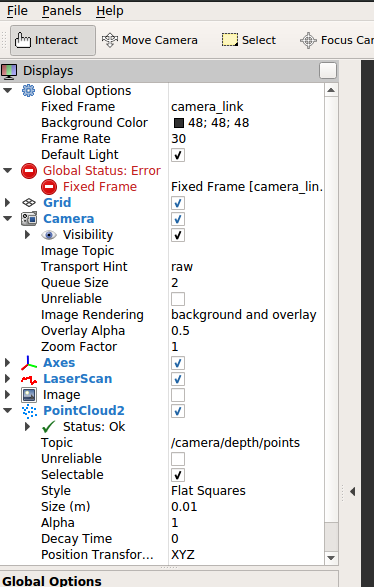
\includegraphics[width=0.3\linewidth]{rviz.png}
\end{center}
\end{frame}


\begin{frame}[fragile,label=sec-4-4]{Visualize data in \texttt{rviz}, contd}
 \begin{center}
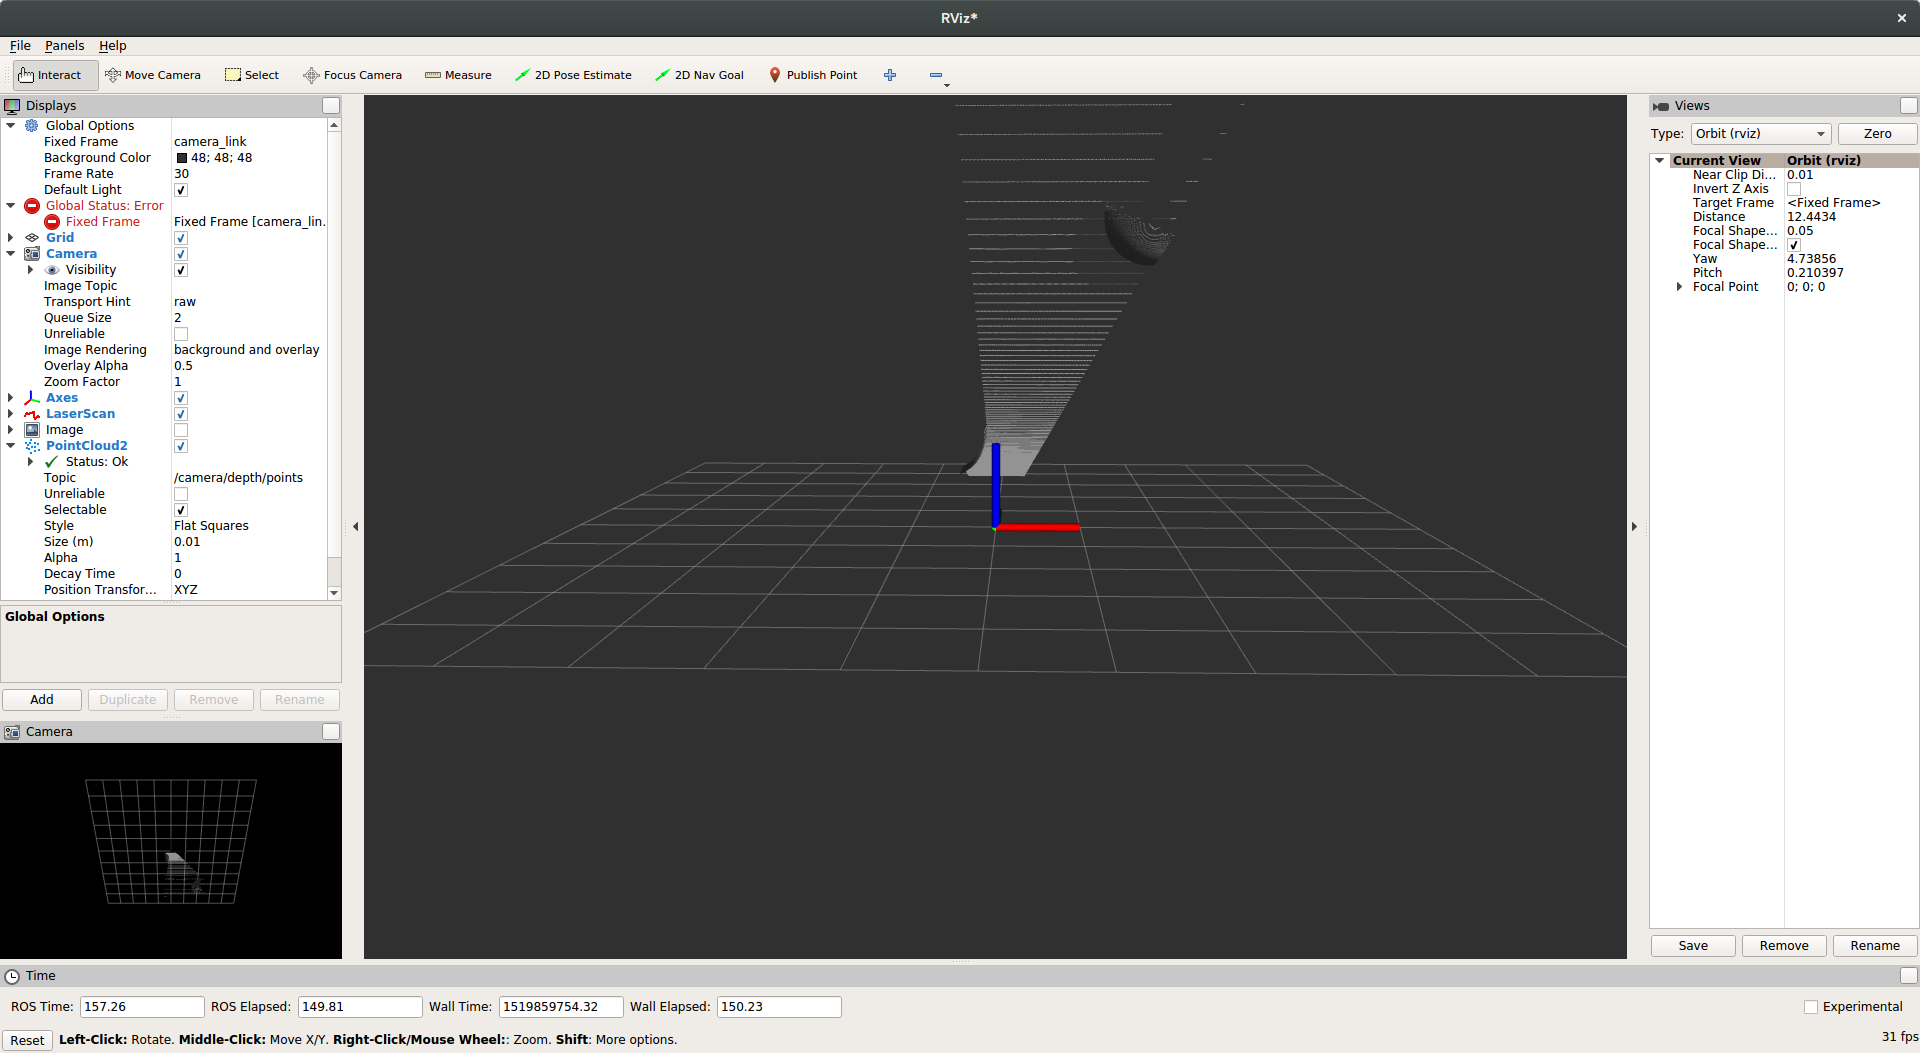
\includegraphics[width=\linewidth]{rviz-view.png}
\end{center}
\end{frame}


\section{Move and watch}
\label{sec-5}

\begin{frame}[fragile,label=sec-5-1]{Look around}
 Make the robot rotate and see the changing view in \texttt{rviz}
\end{frame}

\begin{frame}[fragile,label=sec-5-2]{Look around}
 Make the robot rotate and see the changing view in \texttt{rviz}

\begin{verbatim}
~$ rostopic pub /pioneer2dx/cmd_vel geometry_msgs/Twist \
> '{angular: {z: 0.3}}'
\end{verbatim}
\end{frame}

\section{Using the parameter server}
\label{sec-6}

\begin{frame}[fragile,label=sec-6-1]{The ROS parameter server}
 Which of the following parameters is \alert{not} available (hint: \texttt{rosparam})

\begin{verbatim}
/camera/depth/image_raw/compressed/format
/camera/imager_rate
/gazebo/gravity_x
/gazebo/gravity_y
/gazebo/gravity_z
/gazebo/max_contacts
/gazebo/min_contacts
/gazebo/time_step
/rosdistro
/rosversion
\end{verbatim}
\end{frame}

\begin{frame}[label=sec-6-2]{Setting and getting parameters}
What is the current setting of the gravity vector?
\end{frame}

\begin{frame}[fragile,label=sec-6-3]{Setting and getting parameters, contd}
 \begin{verbatim}
~$ rosparam get /gazebo/gravity_z
-9.8
\end{verbatim}
\end{frame}

\begin{frame}[fragile,label=sec-6-4]{Setting and getting parameters, contd}
 \begin{verbatim}
~$ rosparam set /gazebo/gravity_z -1.62
\end{verbatim}
\end{frame}

\begin{frame}[fragile,label=sec-6-5]{Reading parameters in our own node}
 \begin{verbatim}
...
ros::NodeHandle n;
...

double Kv = 0.1; 
if (n.getParam("Kv", Kv)) {
    ROS_INFO("Setting velocity gain to %f", Kv);
} else {
    ROS_INFO("Velocity gain parameter not found");
}
...
\end{verbatim}
\end{frame}

\begin{frame}[fragile,label=sec-6-6]{Setting parameters in the launch file}
 \begin{verbatim}
<launch>
  <!-- Use the logic in empty_world.launch. Just launch another world -->
  <include file="$(find gazebo_ros)/launch/empty_world.launch">
    <arg name="world_name" value="$(find pioneer_gazebo)/worlds/pioneer-depth-camera.world"/>
    <!-- More params can be changed here -->
  </include>
  <param name="tol" type="double" value="0.2" />
  <param name="Kv" type="double" value="0.05" />
  <param name="Ka" type="double" value="0.1" />
</launch>
\end{verbatim}
\end{frame}

\section{Next steps}
\label{sec-7}
\begin{frame}[label=sec-7-1]{Ideas for future ROS seminars}
\begin{itemize}
\item Point cloud library
\item Navigation
\item ROS control package
\end{itemize}
\end{frame}
% Emacs 24.5.1 (Org mode 8.2.10)
\end{document}